 \documentclass[12pt]{template/iopart}

% allow loading amsmath
\expandafter\let\csname equation*\endcsname\relax
\expandafter\let\csname endequation*\endcsname\relax

\usepackage[english]{babel}
\usepackage{graphicx,helvet}
\usepackage{color}
\usepackage{url}
\usepackage{amssymb}
\usepackage[utf8]{inputenc}
\usepackage[english]{babel}
\usepackage[T1]{fontenc}
\usepackage{hyperref}
\usepackage{graphicx,helvet}
\usepackage{color}
\usepackage[inline]{showlabels}
\usepackage{bbm,bm}
\usepackage{soul}
\usepackage{amsfonts}
\usepackage{iopams}
\usepackage{lipsum}

\usepackage{tikz}
\usetikzlibrary{arrows}
\usetikzlibrary{quantikz}

\usepackage[draft,inline,nomargin]{fixme} \fxsetup{theme=color}
\FXRegisterAuthor{cp}{acp}{\color{blue}CP}
\FXRegisterAuthor{tb}{ttb}{\color{OliveGreen}TB}

\newcommand\keywords[1]{Keywords: #1}








\begin{document}
\title[Title]{Title}

\author{Tomás Basile$^1$ and Carlos Pineda$^2$}

\address{$^1$ Facultad de Ciencias. Universidad Nacional Autónoma de México, Ciudad de México 01000, Mexico}
\address{$^2$ Instituto de Física, Universidad Nacional Autónoma de México, Ciudad de México 01000, México}
\ead{carlospgmat03@gmail.com}

\begin{abstract}
The abstract follows the addresses and
should give readers concise information about the content 
of the article and indicate the main results obtained and conclusions 
drawn. It should be self-contained---there should be no references to 
figures, tables, equations, bibliographic references etc.  It should be enclosed between \verb"\begin{abstract}"
and \verb"\end{abstract}" commands.  The abstract should normally be restricted 
to a single paragraph of around 200 words~\cite{bengtsson_zyczkowski_2017}.
\end{abstract}
\keywords{magnetic moment, solar neutrinos, astrophysics} \\
\submitto{\PS}
\maketitle

\section{Introduction}

To be written later.
\section{Circuits for Pauli Maps}

\begin{itemize}
\item \textbf{Circuit for a Pauli channel:}  Propose a circuit to simulate a Pauli channel on $n$ qubits. It works by creating a $2n$-qubit state on ancilla qubits.
\item \textbf{Simulation:} Show the fidelities of simulating the circuit on a quantum computer for many different one-qubit channels inside the tetrahedron.
\item \textbf{For Pauli dynamical maps}: See how the circuit generalizes to parametrized channels and notice that many rotations are needed to create the $2n$-ancilla qubit state.
\end{itemize}

\section{OPR Circuits}
\begin{itemize}
\item How can we reduce the amount of parametrized rotations used?
\item \textbf{OPR Circuit:} Define an OPR circuit (a circuit with one parametrized rotation)
\item \textbf{Theorem about OPR circuits:} \textit{An OPR circuit on $n$ qubits with parameter $p$ always has an operator of the form:}
\begin{align*}
U = (\vec{v}_0| \vec{v}_1| \cdots| \vec{v}_{2^n-1})
\end{align*}
\textit{where $s = s(p)$ and the column vectors are $\vec{v}_j = e^{is} \vec{a}_j + e^{-is} \vec{b}_j + \vec{c}_j$, with $\vec{a}_j, \vec{b}_j, \vec{c}_j$ orthogonal vectors and $|\vec{a}_j|^2 + |\vec{b}_j|^2 + |\vec{c}_j|^2 = 1$.}
\end{itemize}
\section{OPR circuit for a Pauli map}
\begin{itemize}
\item Use the last theorem to conclude which maps can be created using an OPR circuit.
\item \textbf{Examples:} Show examples that satisfy these conditions: Bit-Flip, parabolic maps, etc. and an example that doesn't satisfy the conditions.
\item \textbf{Results:} Show results of simulating those maps on a quantum computer. 
\end{itemize}
\section{Exponential maps $e^{iHt}$}
\begin{itemize}
\item We will apply the results about OPR circuit to another kind of operation.
\item Consider operations $U  = e^{iHt}$ where $H$ is hermitian  and time independent.
\item \textbf{Theorem:} A n-qubit operator of the form $U = e^{iHt}$ can be implemented using an OPR circuit if and only if the eigenvalues of $H$ are $-\lambda,0,\lambda$ (for $\lambda$ a real number) and the degeneracies of $\lambda$ and $-\lambda$ are $2^j$ for some $j\in \{0,1,\cdots,n-1\}$.
\item \textbf{Examples:} Every matrix $H$ for one qubit, any $n$-qubit pauli matrix, some sums of Pauli matrices, etc.
\end{itemize}
\section{Conclusion}


\newpage
\appendix
\section{Resumen}
\begin{itemize}
\item In this work we study parametrized quantum circuits used to implement
quantum operations over qubit systems. 
\item Specifically, we study two types of operations: Pauli
dynamical maps and transformations of the form $e^{iHt}$ on $n$ qubits. 
\item We focus mainly on operations that can be implemented using a circuit 
with only one parametrized rotation gate (OPR Circuit). 
\item We get the conditions on these operations to be
applied with an OPR circuit:\\

\textbf{Theorem:} An OPR circuit with parameter $p$ on $n$ qubits always has an operator of the form:
\begin{eqnarray}
U  = (\vec{v}_0, \vec{v}_1, \cdots, \vec{v}_{2^n-1})
\end{eqnarray}
where $s = s(p)$ and the column vectors are $\vec{v}_j = e^{is} \vec{a}_j + e^{-is} \vec{b}_j + \vec{c}_j$, with $\vec{a}_j, \vec{b}_j, \vec{c}_j$ orthogonal vectors and $|\vec{a}_j|^2 + |\vec{b}_j|^2 + |\vec{c}_j|^2 = 1$. \\

\item We propose a circuit to simulate Pauli dynamical maps on $n$ qubits using $2n$ ancilla qubits. We find the conditions for channels that can be simulated by an OPR circuit and some examples that fulfill these conditions. 

\item We find the conditions that a matrix $H$ must have for the operation $e^{iHt}$ to be implementable with an OPR circuits: \\

 \textbf{Theorem:} An $n-$qubits operator $U = e^{iHt}$ (with $H$ time-independent) can be implemented using an OPR circuit if and only if the eigenvalues of $H$ are $-\lambda, 0, \lambda$ (for $\lambda$ a real number) and the degeneracies of $\lambda$ and $-\lambda$ are $2^j$ for some $j$ such that $0 \leq j <n$.
\item We find how to construct the OPR circuit that implements $e^{iHt}$ given the conditions of the theorem and see some examples. 

\item Finally, we implement some of these
circuits on IBM's quantum computers and obtain their fidelities.
\end{itemize}
\newpage


\section{Partes más desarrolladas}
\subsection{Resumen}
In this work we study parametrized quantum circuits used to 
implement quantum operators over qubits systems on a quantum computer. 
Specifically, we study Pauli dynamical maps and unitary transformations of the form $e^{iHt}$.
 We focus mainly on operations that can be implemented using a circuit  with only one parametrized rotation gate (OPR circuit),
 and get the conditions these operations must satisfy for 
 being applicable on an OPR circuit.
Finally, we implemented some specific examples of these circuits on IBM's quantum computers
and obtain the fidelity of this implementation.

\subsection{Introduction}
\begin{itemize}
\item 
\end{itemize}

\subsection{OPR Circuits}

\textbf{Definition, Circuit with one parametrized Gate (OPR circuit):} A quantum circuit
 that contains only one gate that depends on a parameter $p$.
Furthermore, the parametrized gate is a one qubit rotation about any axis. \\

\textbf{Property 1:} \textit{An $n$-qubit OPR circuit can always be transformed into the form of circuit \ref{fig: OPR general-A}, where $A$ and $B$ are $n$-qubit gates that don't depend on the parameter
and $s = s(p)$ is a function of the parameter.}\\

\begin{figure}[h!]
\centering
\begin{quantikz}
\lstick{$q_0$} & \qw & \gate[wires = 4,nwires=3]{B} & \ctrl{3} & \qw & \gate[wires=4,nwires=3]{A} & \qw \\
\lstick{$q_1$} & \qw &  & \ctrl{2} & \qw & & \qw \\
\vdots & \vdots & & & \vdots & \\
\lstick{$q_{n-1}$} & \qw & & \gate{R_{\sigma_3}(2s(p))} & \qw & & \qw
\end{quantikz}
\caption{Forma general de un circuito RP.}
\label{fig: OPR general-A}
\end{figure}

First of all, we notice that by definition an OPR
will always consist on some operation $B$ followed by the parametrized rotation 
and then some operation $A$, where $A$ and $B$ are not parametrized. 

Then, we notice that it isn't necessary to consider rotations
about an arbitrary axis, since a rotation about $\hat{n}$ parametrized by $p$ can
be converted into a rotation about $\sigma_3$ without the need of introducing gates that depend on $p$.
To see this, consider the rotation $R_{\hat{n}}(2s)$, where $2s$ is some function of $p$ (the $2$ is added for convenience later on) and $\hat{n} = (n_1,n_2,n_3)$ is the rotation axis,
 which can be written as $(n_1,n_2,n_3) = (\sin \theta \cos \phi , \sin \theta\sin \phi, \cos \theta)$ for some fixed angles $\phi, \theta$ dependent on $\hat{n}$. 
 Then, the rotation can be rewritten as (ref 12 de la tesis):
\begin{eqnarray}
R_{\hat{n}}(2s) = R_{\sigma_3}(\phi) R_{\sigma_2}(\theta) R_{\sigma_3}(2s) R_{\sigma_2}(-\theta) R_{\sigma_3}(-\phi).
\end{eqnarray}
Because angles $\theta, \phi$ don't depend on the parameter $p$, 
any OPR circuit can be converted into a circuit in which the parametrized rotation is around $\sigma_3$ instead of an arbitrary axis.

Furthermore, the qubit to which the rotation is applied can be selected to be the last one,
since otherwise  swap gates can be added before and after the rotation to make it act on the last qubit.

Therfore, an OPR circuit can be transformed in a way that the rotation is around $\sigma_3$ and applied on the last qubit 
(possibly controlled by other qubits), 
so that it has the form \ref{fig: OPR general-A}. $\blacksquare$ \\

\textbf{Property 2:} \textit{An OPR circuit implements an operator with a matrix in the computational basis of the form:}
\begin{eqnarray}
U = (|\vec{v}_0|, |\vec{v}_1|, |\vec{v}_2|, \cdots, |\vec{v}_{2^n-1}|),
\end{eqnarray}
\textit{where the column vectors are $\vec{v}_j = e^{is} \vec{a}_j + e^{-is} \vec{b}_j + \vec{c}_j$,
with $\vec{a}_j ,\vec{b}_j, \vec{c}_j$ orthogonal and $|\vec{a}_j|^2 + |\vec{b}_j|^2 + |\vec{c}_j|^2 = 1$.}\\

\textbf{Proof:} Because of property 1, we know that any OPR
circuit can be converted into the form \ref{fig: OPR general-A},
so that we only need to consider the operator for that circuit. 
The $j$-th column of the circuit's matrix will be the result of applying the 
circuit to the state $|j\rangle$. 
First, applying $B$ to that state results in $B_{0,j} |0\rangle |0\rangle + B_{1,j} |1 \rangle + \cdots + B_{2^n-1,j}|2^n-1\rangle$,
 which can be rewritten by separating the states to which the controlled 
rotation will be applied from those to which it won't as follows:
\begin{eqnarray}
\sum_{k \in Ctrl} \left(B_{2k,j} |k\rangle |0\rangle + B_{2k+1,j} |k\rangle |1 \rangle \right) + \sum_{k \not\in Ctrl} \left( B_{2k,j} |k\rangle |0\rangle + B_{2k+1,j}|k\rangle |1\rangle \right),
\end{eqnarray}
where $Ctrl$ is the set of all basis states of the first $n-1$ qubits
such that they fulfill the controls of the rotation gate and therefore the gate is applied.

After $B$ creates this state, we need to apply the rotation to the result. 
This rotation will only be applied for those states on the first sum (since the fulfill the control conditions)
and not to the others. Therefore, we apply the gate to the last qubit of these states, 
remembering that $R_z(2s)$ acts by just adding a phase $e^{-is}$ to the $|0\rangle$ state
and a phase $e^{is}$ to the $|1\rangle$ state, and the result is:
\begin{eqnarray}
& e^{-is} \sum_{k \in Ctrl} B_{2k,j} |k\rangle |0\rangle + e^{is} \sum_{k \in Ctrl} B_{2k+1,j} |k\rangle |1 \rangle + \sum_{k \not\in Ctrl} \left( B_{2k,j} |k\rangle |0\rangle + B_{2k+1} |k\rangle |j \rangle \right)\\
& \qquad := e^{-is} \vec{b'}_j + e^{is} \vec{a'}_j + \vec{c'}_j,
\end{eqnarray}
where $\vec{a'} = \sum_{k \in Ctrl} B_{2k,j}|k\rangle|0\rangle \;,\; \vec{b'}_j = \sum_{k \in Ctrl} B_{2k+1,j} |k\rangle |1 \rangle \;,\; \vec{c'}_j =\sum_{k \not\in Ctrl} \left( B_{2k,j} |k\rangle |0\rangle + B_{2k+1} |k\rangle |j \rangle \right) := e^{-is} \vec{b'}_j + e^{is} \vec{a'}_j + \vec{c'}_j$.
 These vectors are clearly orthogonal because they are each linear combinations of different orthogonal states of the computational basis. 
Moreover, they satisfy $|\vec{a'}_j|^2 + |\vec{b'}_j|^2 + |\vec{c'}_j|^2 = 1$ because this quantity is the norm of the $j-$th column of $B$.

Finally, after having applied the rotation, the circuit applies gate $A$, 
so that the result is given by:
\begin{eqnarray}
e^{-is} A \vec{a'}_j + e^{is} A \vec{b'}_j + A \vec{c'}_j := e^{-is} \vec{a}_j + e^{is} \vec{b}_j + \vec{c}_j := \vec{v}_j,
\end{eqnarray}
where $\vec{a}_j = A \vec{a'}_j , \vec{b}_j = A \vec{b'}_j , \vec{c}_j = A \vec{c'}_j$ are orthogonal
vectors that satisfy $|\vec{a}_j|^2 + |\vec{b}_j|^2 + |\vec{c}_j|^2 = 1$ because $A$ is unitary. 
Therefore, we conclude that the circuit takes a state $|j\rangle$ and converts it
 into the state represented by the vector $\vec{v}_j$, which means that the matrix representation of the circuit's operation is
 $U = (|\vec{v}_0|, |\vec{v}_1|, \cdots, |\vec{v}_{2^n-1}|)$. \\
\subsection{Pauli Channels and maps}
\subsubsection{Basic Definitions}

\begin{itemize}
\item A system of n-qubits can be represented by a positive matrix $\rho$ of size $2^n \times 2^n$ called the density matrix.
\item  An important set of operators acting on these systems are the Pauli operators, which are defined as
\begin{eqnarray}
\sigma_{\vec{\alpha}} = \sigma_{\alpha_1} \otimes \sigma_{\alpha_2} \otimes \cdots \otimes \sigma_{\alpha_n},
\end{eqnarray}
where $\vec{\alpha} = (\alpha_0, \alpha_1, \cdots , \alpha_{n-1})$ , $\alpha_i \in \{0,1,2,3\}$ and $\sigma_{\alpha_i}$ is the $\alpha_i$-th one qubit Pauli operator. \\

\item Using these operators, we define a Pauli channel as a transformation of the density matrix given by
\begin{eqnarray}
\varepsilon(\rho) = \sum_{\vec{\gamma}} k_{\vec{\gamma}} \sigma_{\vec{\gamma}} \rho \sigma_{\vec{\gamma}} ,
\end{eqnarray}
where $k_{\vec{\gamma}}$ are positive real numbers such that $\sum_{\vec{\gamma}} k_{\vec{\gamma}} = 1$ (necessary conditions for the channel $\varepsilon$ to be completely positive and trace preserving).\\
\end{itemize}

\subsubsection{Circuit for a Pauli Channel}

We are interested in finding a way to construct a quantum circuit that can implement an arbitrary Pauli channel on a system of $n$ qubits. To do it, it is important to realize that a Pauli channel $\varepsilon (\rho) = \sum_{\vec{\gamma}} k_{\vec{\gamma}} \sigma_{\vec{\gamma}} \rho \sigma_{\vec{\gamma}}$ can be interpreted as an statistical mixture of the Pauli operators $\sigma_{\vec{\gamma}}$ applied to the density matrix $\rho$  with  probabilities $k_{\vec{\gamma}}$. That is, it can be interpreted as a transformation that applies each Pauli operator $\sigma_{\vec{\gamma}}$ on $\rho$ with a probability $k_{\vec{\gamma}}$.

Given this interpretation of the channel, it is easy to construct a quantum circuit that implements it with the help of $2n$ ancilla qubits. The general idea is to first construct a state on the ancilla qubits and then use this state and controlled gates to  apply each Pauli operator $\sigma_{\vec{\gamma}}$ with probability $k_{\vec{\gamma}}$ on the principal qubits. 

The circuit that does this is presented in figure \ref{fig: circuito-A}, where $|\vec{\gamma}\rangle$ is defined as the $2n$ qubits state $|\vec{\gamma} \rangle = \otimes_{i=0}^n |\gamma_i \; \text{in binary} \rangle$. For example, if $\vec{\gamma} = (0,3,1,\cdots)$, then this state is defined as $|\vec{\gamma} \rangle = |001101 \rangle$.

\begin{figure}[h!]
\centering
\begin{quantikz}
\lstick{$q_0$} & \qw & \qw & \qw & \gate{\sigma_{\gamma_0}} & \qw & & &  & & \rstick[wires=12]{Repeat for all \\
 vectors $\vec{\gamma}$} \\
\lstick{$q_1$} & \qw & \qw & \qw & \gate{\sigma_{\gamma_1}} & \qw & & & &\\
\lstick{ } & \vdots & \vdots & \vdots & &  & & & &\\
\lstick{$q_{n-1}$} & \qw & \qw & \qw & \gate{\sigma_{\gamma_{n-1}}} & \qw & & &\\
\lstick{ } & & & & & &\\
\lstick{$aq_0$} & \qw & \gate[wires=7,nwires=5]{\text{Create the $2n$ qubits state $\sum_{\vec{\gamma}} \sqrt{k_{\vec{\gamma}}}   |\vec{\gamma} \rangle$}} & \qw &  \ctrl{-5} & \qw & \rstick[wires=2]{$|\gamma_0 \rangle$} &  & & &\\
\lstick{$aq_1$} & \qw & & \qw &  \ctrl{-6} &\qw & & & & & \\
\lstick{$aq_2$} &\qw & & \qw &  \ctrl{-7} & \qw & \rstick[wires=2]{$|\gamma_1 \rangle$} & & & &\\
\lstick{$aq_3$} &\qw & & \qw &  \ctrl{-8} & \qw & & & & &\\
\vdots  &\vdots & & \vdots & &  \vdots & & & & &\\
\lstick{$aq_{2n-2}$}& \qw &  &\qw  & \ctrl{-10} & \qw & \rstick[wires=2]{$|\gamma_{n-1} \rangle$}& & & & \\
\lstick{$aq_{2n-1}$}& \qw & & \qw  &  \ctrl{-11} & \qw & & & & &\\
\end{quantikz}
\caption{Circuit for a n-qubit Pauli channel.}
\label{fig: circuito-A}
\end{figure}

Where 

\begin{figure}[h!]
\centering
\begin{quantikz}
& \ctrl{1} & \qw \rstick[wires=2]{$|\gamma_i \rangle$} \\
& \control{} & \qw
\end{quantikz}
\end{figure}
indicates that the controlled gate is activated if these two qubits are in the state $|\gamma_i \rangle$. In particular, using the common notation for controlled gates, we have
\begin{figure}[h!]
\centering
\begin{quantikz}
& \octrl{1} & \qw \rstick[wires=2]{if $\gamma_i = 0$} \\
& \ocontrol{} & \qw
\end{quantikz} \begin{quantikz}
& \octrl{1} & \qw \rstick[wires=2]{if $\gamma_i = 1$} \\
& \control{} & \qw
\end{quantikz}  \begin{quantikz}
& \ctrl{1} & \qw \rstick[wires=2]{if $\gamma_i = 2$} \\
& \ocontrol{} & \qw
\end{quantikz}  \begin{quantikz}
& \ctrl{1} & \qw \rstick[wires=2]{if $\gamma_i = 3$} \\
& \control{} & \qw
\end{quantikz}
\end{figure}

To see why this circuit works, we note that after creating the state $\sum_{\vec{\gamma}} \sqrt{k}_{\gamma} \; |\vec{\gamma} \rangle$, the circuit applies each gate $\sigma_{\vec{\gamma}}$ to the principal qubits under the condition that the ancilla qubits are on the state $|\vec{\gamma}\rangle$. This  means that each gate $\sigma_{\vec{\gamma}}$ is applied on the principal qubits with a probability $\sqrt{k_{\vec{\gamma}}}$, just as we wanted.  \\

\subsubsection{Pauli Dynamical Maps}

A Pauli dynamical map is defined as a continuous parametrized curve drawn inside the set of Pauli channels and starting at the identity channel. Therefore, a Pauli dynamical map can be written as
\begin{eqnarray}
\varepsilon_p(\rho) = \sum_{\vec{\gamma}} k_{\vec{\gamma}}(p) \sigma_{\vec{\gamma}} \rho \sigma_{\vec{\gamma}},
\end{eqnarray}
where $p$ is a parameter belonging to an interval $[a,b]$ and $\varepsilon_p$ is a Pauli channel for every $p$, with $\varepsilon_a$ being the identity channel.

Dynamical maps can be implemented using the same method as in figure \ref{fig: circuito-A}, with the only difference that now the state to be created on the ancilla qubits depends on parameter $p$ and it is given by $\sum_{\vec{\gamma}} \sqrt{k_{\vec{\gamma}}(p)} |\vec{\gamma}\rangle$.  \\

\subsubsection{OPR Circuit for dynamical maps}

For OPR circuits, the ancilla state has to be created with only one parametrized curve. Then, the theorem for OPR circuits implies that a map
\begin{eqnarray}
\varepsilon_p(\rho) = \sum_{\vec{\gamma}} k_{\vec{\gamma}}(p) \sigma_{\vec{\gamma}} \rho \sigma_{\vec{\gamma}},
\end{eqnarray}
can be implemented  if there are numbers $\beta_{\vec{\gamma}}(p)$ such that $|\beta_{\vec{\gamma}}(p)|^2 = k_{\vec{\gamma}}(p)$ and
\begin{eqnarray}
\sum_{\vec{\gamma}} \beta_{\vec{\gamma}}(p) |\vec{\gamma}\rangle = \vec{c} + \vec{a} \cos s + \vec{b} \sin s
\end{eqnarray}
where $\vec{a},\vec{b},\vec{c}$ are orthogonal vectors in $\mathbb{C}^{2n}$ and $|\vec{a}|^2+  |\vec{b}|^2 + |\vec{c}|^2= 1$.

\subsubsection{Examples on one qubit and implementation on IBM computers}

For the special case of a system consisting of only one qubit, a Pauli channel takes the form
\begin{eqnarray}
\varepsilon(\rho) = k_0 I \rho I + k_1 X \rho X + k_2 Y \rho Y + k_3 Z \rho Z,
\end{eqnarray}
and the circuit that can be used to implement it reduces to:
\begin{figure}[h!]
\centering
\begin{quantikz}
\lstick{$q_0$} & \qw & \gate{\sigma_1} & \gate{\sigma_2} & \gate{\sigma_3} & \qw \\
\lstick{$aq_0$} & \gate[wires=2][3cm]{\quad\quad \text{Create the two qubits state}\quad\quad} & \octrl{-1} & \ctrl{-1} & \ctrl{-1} & \qw \\
\lstick{$aq_1$} & \gateinput{$\sqrt{k_0} |0 \rangle |0 \rangle + \sqrt{k_1} |0 \rangle |1 \rangle + \sqrt{k_2} |1 \rangle |0 \rangle + \sqrt{k_3} |1 \rangle |1 \rangle $} & \ctrl{-2} & \octrl{-2}  & \ctrl{-2} & \qw
\end{quantikz}
\caption{ Circuit for a one qubit Pauli channel.}
\label{fig: canal-1qbit-A} 
\end{figure}

This circuit can be applied for any one-qubit Pauli channel. It is well known that these channels can be represented as points in a tetrahedron with corners $(1,1,1)$, $(1,-1,-1)$, $(-1,1,-1)$ and $(-1,-1,1)$. To put the circuit to test, we sampled $250$ points inside the tetrahedron and applied quantum process tomography to each one by using Qiskit's ibmq-lima quantum computer. The fidelity of the Choi matrix obtained by quantum process tomography with respect to the theoretical Choi matrix of each channel was calculated and is plotted in the next figure. 



\begin{figure}[h!]
\centering
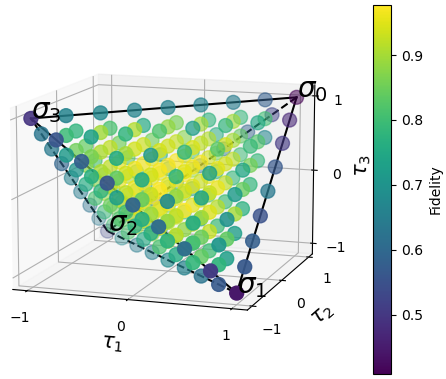
\includegraphics[width=0.45\textwidth]{fidelity-points.png}\\
\caption{Fidelity of one qubit channels using Qiskit's ibmq-lima.}
\end{figure}


\paragraph{$\sigma_3$ parabolic map} $\;$ \\

We take as an example the Pauli dynamical map for one qubit defined as
\begin{eqnarray}
\epsilon(\rho) = \dfrac{1}{4} (1-p)^2 \sigma_0 \rho \sigma_0 + \dfrac{1}{4} (1-p^2) \sigma_1 \rho \sigma_1 + \dfrac{1}{4} (1-p^2) \sigma_2 \rho \sigma_2 + \dfrac{1}{4} (1+p)^2 \sigma_3 \rho \sigma_3 ,
\end{eqnarray}
with $p \in [-1,1]$. \\

To implement this dynamical map using the circuit presented in figure \ref{fig: one-rot-A}, it is necessary to create the state
\begin{eqnarray}
\left(\dfrac{1}{2} (1-p) , \dfrac{1}{2} \sqrt{1-p^2} , \dfrac{1}{2} \sqrt{1-p^2} , \dfrac{1}{2}(1+p) \right)
\end{eqnarray}
on the $2$ ancilla qubits. Luckily, this state can be written in the form $\vec{c} + \vec{a} \cos s + \vec{b} \sin s$ as
\begin{eqnarray}
\begin{pmatrix}
1/2 \\
0 \\ 
0 \\
1/2
\end{pmatrix} + \begin{pmatrix}
0 \\
1/2 \\
1/2 \\
0
\end{pmatrix}  \cos s + \begin{pmatrix}
-1/2 \\
0 \\
0 \\
1/2
\end{pmatrix} \sin s
\end{eqnarray}
with $s = \arcsin p$. According to theorem 1, the fact that the state we need to create over the ancilla qubits can be written like this implies that the dynamical map can be simulated in a quantum computer using only one parametrized rotation. The circuit used will have the same form as that in figure \ref{fig: canal-1qbit-A}, where the part used to create the state on the ancilla qubits will be:
\begin{figure}[h!]
\centering
\begin{quantikz}
\lstick{$aq_0$} & \gate[wires=2]{B} & \ctrl{1} & \gate[wires=2]{A} & \qw \\
\lstick{$aq_{1}$} & & \gate{R_{\sigma_2}(2s)} & & \qw  \\
\end{quantikz}
\caption{Circuit to create 2-qubit state}
\end{figure}

where according to theorem 1, matrices $A$ and $B$ can be chosen as:
\begin{eqnarray}
A &= \begin{pmatrix}
*  & c_0 / \sqrt{1-r^2} & -b_0/r & a_0 /r \\
*  & c_1 / \sqrt{1-r^2} & -b_1/r & a_1 /r \\ 
* & c_2 / \sqrt{1-r^2} & -b_2/r & a_2/r \\
* & c_3 / \sqrt{1-r^2} & -b_3/r & a_3/r \\
\end{pmatrix} = \begin{pmatrix}
0 & 1/\sqrt{2} & -1/\sqrt{2} & 0 \\
-1/\sqrt{2} & 0 & 0 & 1/\sqrt{2} \\
1/\sqrt{2} & 0 & 0 & 1/\sqrt{2} \\
0 & 1/\sqrt{2} & 1/\sqrt{2} & 0
\end{pmatrix} \\
B& = \begin{pmatrix}
0 & 0 & 0 & 1 \\
0 & 1 & 0 & 0\\
0 & 0& 1 & 0 \\
1 & 0 & 0 & 0 
\end{pmatrix}
\end{eqnarray}


To put it to test, we selected $20$ equally spaced values of $p$ between $-0.9$  and $0.9$ and implemented the corresponding circuit using the ibmq-Lima quantum computer. For each point, we used quantum process tomography to obtain the Choi matrix for the channel. Then, we calculated the fidelity of this matrix with respect to the theoretical Choi matrix of the channel. The following figure shows the fidelity of the simulated circuit for each value of $p$.
\begin{figure}[h!]
\centering
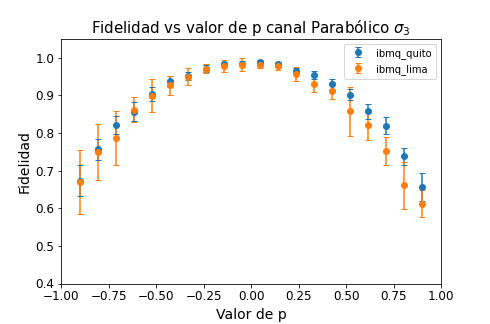
\includegraphics[width=0.55\textwidth]{fidelity-parabolic.PNG} \\
\caption{Fidelity for the Parabolic channel.}
\end{figure}


\newpage
\subsection{Unitary evolution $U = e^{iHt}$}
\section{Exponential maps $e^{iHt}$} % {{{
\label{sec: Exponential maps}
\textbf{Puntos:}
\begin{itemize}
\item We will apply the results about 1PR circuit to another kind of operation, those given by $U  = e^{iHt}$ where $H$ is hermitian  and time independent.
\item \textbf{Lemma:}\textit{ The $n$-qubit operator $U^{iHt}$ can be implemented with a 1PR circuit of $n$ qubits if and only if $D = \text{diag}(e^{i\lambda_0 t}, \cdots, e^{i \lambda_{2^n-1}t})$ can be implemented with a 1PR circuit of $n$ qubits, where $\lambda_j$ are the eigenvalues of $H$.}
\item \textbf{Proof:}  Es b\'asicamente usar que $H = QDQ^{-1}$ para una matriz $Q$ que no depende de $t$ y por lo tanto no agrega compuertas parametrizadas al circuito. 
\item \textbf{Theorem:} \textit{ A n-qubit operator of the form $U = e^{iHt}$ can be implemented using a 1PR circuit if and only if the eigenvalues of $H$ are $-\lambda,0,\lambda$ (for $\lambda$ a real number) and the degeneracies of $\lambda$ and $-\lambda$ are both equal to $2^j$ for some $j\in \{0,1,\cdots,n-1\}$.}
\item \textbf{Proof:} Estoy buscando formas de simplificar la prueba, porque es medio larguita. Pero básicamente es usar el lema y entonces preocuparnos sólo por $D$. Luego  usar el teorema de la sección 3 y notar que sólo hay tres tipos de  $\lambda$s posibles y luego notar que deben de tener esas degeneraciones.
\item \textbf{Proof del regreso:} Aquí quiero recalcar que la prueba es constructiva, ya que consiste en mostrar cómo construir el circuito 1PR que hace la operación a partir de una $H$ que cumpla la hipótesis. 
\item \textbf{Examples.} Mencionar que por el teorema, los ejemplos son sistemas con 3 energías separadas por la misma distancia y con las degeneraciones dadas en el teorema. 
La verdad que no se me ocurren sistemas físicos comunes que cumplan eso.
\begin{itemize}
\item Cualquier matriz $H$ de un qubit cumple el teorema.
\item Cualquier matriz de $n$ qubits que sea el producto tensorial de matrices de Pauli para cada partícula (o sea algo como $\sigma_{i_1} \otimes \sigma_{i_2} \otimes \cdots \otimes \sigma_{i_n}$) cumple el teorema.
\item Estoy viendo para cadenas de espines si hay condiciones para las que cumplan las hipótesis del teorema, pero no he encontrado aún.
\end{itemize}
\item Hice explícitamente el circuito de 2 qubits para $H = \sigma_3 \otimes \sigma_2$ y lo simulé en las computadoras de IBM, obteniendo una fidelidad de $0.85$.
\end{itemize}
% }}}
\newpage

We are now interested on what conditions must an $n$-qubit time independent Hamiltonian $H$
fulfill for the unitary operator $U = e^{iHt}$ to be
implementable with an OPR circuit of $n$ qubits. \\


\textbf{Lemma:} \textit{The $n$-qubit operator $U = e^{iHt}$ can be implemented with an OPR circuit of $n$ qubits
if and only if $D = diag(e^{i\lambda_0 t}, \cdots, e^{i\lambda_{2^n-1}t})$ can be implemented with an OPR circuit of $n$ qubits,
where $\lambda_j$ is the $j$-th eigenvalue of $H$}\\

\textbf{Proof:} The hamiltonian $H$ can be diagonalized as $QHQ^{-1} = diag(\lambda_0,\lambda_1, \cdots,\lambda_{2^n-1})$
 where $Q$ is the  change of  basis matrix and doesn't depend on the parameter $t$ 
 (because $H$ is time independent). Then, the unitary matrix $U = e^{iHt}$ can be diagonalized similarly as $D = QUQ^{-1}$ where $D = diag(e^{i\lambda_0 t}, \cdots, e^{i\lambda_{2^n-1}t})$.
 
Then, if we have an OPR circuit for $U = e^{iHt}$, adding $Q$ and $Q^{-1}$ before and after the circuit converts it into an OPR circuit that
implements $D$. On the other hand, given an OPR circuit for $D$, adding $Q^{-1}$ and $Q$ before and after
converts it into an OPR circuit for $U$. $\blacksquare$. \\


\textbf{Theorem:} \textit{A $n$-qubits operator of the form $U = e^{iHt}$ (where $H$ is time independent) can be implemented 
using an OPR circuit if and only if the eigenvalues of $H$
are $-\lambda, 0, \lambda$ (for $\lambda$ a real number) and the degeneracy of $\lambda$ and $-\lambda$ is $2^j$ for $0 \leq j < n$.} \\

\textbf{Proof:} According to the lemma, if $U = e^{iHt}$ is implementable using an $n$-qubit OPR circuit,
then the diagonal matrix $D = diag(e^{i\lambda_0 t}, \cdots, e^{i\lambda_{2^n-1}t})$ is implementable using an $n$-qubit OPR circuit too,
 where $\lambda_k$ are the eigenvalues of $H$. 

Therefore, according to Property 2 of OPR circuits,
matrix $D$ must have the form $(|\vec{v}_0|, |\vec{v}_1|, \cdots , |\vec{v}_{2^n-1}|)$, 
but because $D$ is diagonal, this form reduces to:
\begin{eqnarray}
D = \begin{pmatrix}
c_{00} + a_{00} e^{is} + b_{00} e^{-is} & 0 & \cdots  \\
0& c_{11} + a_{11} e^{is} + b_{11} e^{-is} & \cdots  \\
 \cdots & \cdots & \ddots 
\end{pmatrix}.
\end{eqnarray}
Furthermore, the column vectors $\vec{a}_j, \vec{b}_j, \vec{c}_j$ must be orthogonal, but because each column has only one nonzero entry,
only one of the vectors can be nonzero, so each entry must be $c_{jj}$ or $a_{jj} e^{is}$ or $b_{jj} e^{-is}$. 
And because the vectors also satisfy $|\vec{a}_j|^2 + |\vec{b}_j|^2 + |\vec{c}_j|^2 = 1$, it must be true that $|c_{jj}|^2 = 1 $
or $|a_{jj}|^2 = 1$ or $|b_{jj}|^2 =1$.
Therefore, the $j$-th entry in the diagonal matrix must be of the form $e^{i \theta_{j}}$ or
$e^{i \theta_{j}} e^{is}$ or $e^{i \theta_j} e^{-is}$. Consequently, we can define the following sets:
\begin{eqnarray}
\Lambda_c = \{\lambda_j  | e^{i\lambda_j t} = e^{i \theta_j}\} \; ,\;
\Lambda_a = \{\lambda_j  | e^{i\lambda_j t} = e^{i \theta_j + is}\} \;,\;
\Lambda_b = \{\lambda_j  | e^{i\lambda_j t} = e^{i \theta_j-is}\}.
\end{eqnarray}
Every eigenvalue must belong to one of these sets. We can prove the following properties of these sets:
\begin{itemize}
\item The only eigenvalues in $\Lambda_c$ are $\lambda_j = 0$: This is because  $e^{i \lambda_j t}  = e^{i \theta_j}$ for every $t$ implies that $\lambda_j = 0$.
\item All eigenvalues in $\Lambda_a$ ($\Lambda_b)$ have the same value:
Take $\lambda_k , \lambda_j \in \Lambda_a (\Lambda_b)$, then $e^{i\lambda_k t} = e^{i \theta_k \pm is} \; ,\; e^{i\lambda_j t} = e^{i\theta_j \pm is}$,
therefore $\lambda_k t = \theta_k \pm s + 2\pi n_k$ and $\lambda_j t = \theta_j \pm s + 2\pi n_j$ with $n_k, n_j$ integers.
 Subtracting these equations implies that $(\lambda_k - \lambda_j)t = \theta_k - \theta_j + 2\pi n_k - 2\pi n_j$. 
 Given that the right side doesn't depend on $t$, we conclude that $\lambda_k - \lambda_j= 0$, so the eigenvalues are the same.
 
\item Eigenvalues in $\Lambda_a$ and $\Lambda_b$ have the same magnitude but opposite sign: 
Take an eigenvalue $\lambda_j \in \Lambda_a$ and $\lambda_k \in \Lambda_b$, 
then just as in the last step, we conclude that $\lambda_jt =  \theta_j + s + 2\pi n_j$ and $\lambda_kt = \theta_k - s + 2\pi n_k$
and adding these equations we get $(\lambda_j+ \lambda_k)t = \theta_j + \theta_k + 2\pi (n_j + n_k)$. 
Given that the right side doesn't depend on $t$, we conclude that $\lambda_j + \lambda_k =0$, so that $\lambda_j$ and $\lambda_k$ have opposite signs but equal magnitude.
\end{itemize}
Therefore, we conclude that the eigenvalues can be chosen out of $H$ must be chosen 3 sets, 
those in $\Lambda_c$ are equal to $0$, those in $\Lambda_a$ are equal to a value we
will call $\lambda$ and those in $\Lambda_b$ are all equal to $-\lambda$. 

Finally, we notice that the degeneracy of $\lambda$ and
$-\lambda$ are $2^j$ for some $j \in \{0, \cdots, n-1\}$.
 To see that, we remember that because it is an OPR circuit, 
Matrix $D$ is equal to $D = A R_{\sigma_3} (2s)B$, 
with $R_{\sigma}$ a rotation applied to the last qubit and controlled by set of the first qubits and $A,B$ 
matrices that don't depend on $s$.
Furthermore, the matrix $R_{\sigma_3}(2s)$ is diagonal and
it has $2^j$ entries equal to $e^{is}$, $2^j$ entries equal to $e^{-is}$ and the rest equal to $1$ 
(where $j+1$ is the number of  control qubits). 
Therefore, we can write $R_{\sigma_3}(2s) = M_1 + e^{is} M_+ + e^{-is} M_-$
 where $M_1, M_+, M_-$ are diagonal matrices with all non-zero entries equal to $1$ and 
$M_+, M_-$ has $2^j$ non-zero entries and $M_1$ has $2^n - 2^{j+1}$ non-zero entries.

Finally, $D = A(M_1 + e^{is} M_+ + e^{-is} M_-) B = AM_1 B + e^{is} AM_+ B + e^{-is} AM_- B$,
and because $D$ is diagonal, $AM_1B , e^{is} AM_+B, e^{-is} AM_- B$ are
diagonal too. Due to the $A$ and $B$ being full-rank matrices, $e^{is} AM_+B$ 
and $e^{-is} AM_-B$ have a rank of $2^j$ and $AM_1B$ has a rank of $2^n- 2^{j+1}$. 
Therefore, considering $D$ is full rank and diagonal, 
$2^j$ of its entries will be $e^{is}$, another $2^j$ will be $e^{-is}$
and the rest will be $1$. \\

\textbf{Constructing the 
Circuit:}  Given that $H$ has the form given in the theorem,
then $e^{iHt}$ can be diagonalized as $D = diag(e^{i\lambda_0 t}, \cdots , e^{i\lambda_{2^n-1}t})$,
where $2^j$ of the entries are $e^{i\lambda t}$, another $2^j$ are $e^{-i\lambda t}$ 
and the rest are $1$. 
Given a value of $j$, we construct a rotation $R_{\sigma_3}(2\lambda t)$ on the last qubit and with $n-1-j$ control qubits 
(whichever we choose, as long as they are $n-1-j$).
Therefore, the matrix representing this rotation is diagonal with $2^j$
entries being $e^{i\lambda t}$, another $2^j$ being $e^{-i\lambda t}$ and the rest being $1$.
This matrix can then be multiplied by matrices that don't depend on $t$
such that the eigenvalues are reordered and we get the matrix $D$.
That it, we can get matrix $D$ using only one rotation that depends on $t$. 
Then, because $U = Q^{-1} D Q$, we can add matrices $Q^{-1}$ and $Q$ to the circuit
to obtain the complete OPR circuit of $U$. $\blacksquare$ \\ 

\textbf{Note:} If we don't care about adding a global phase to the circuit, the eigenvalues can be translated to $-\lambda+a, a, \lambda+a$ for some $a\in \mathbb{R}$.\\

\subsubsection{Example}
\begin{itemize}
\item  Every matrix $H$ of $n$ qubits obtained as the
tensor product of $n$ Pauli operators fulfills the conditions of the theorem, 
because in particular all eigenvalues of $H$ will
be $1$ or $-1$ with the same number of each. 
\item Every matrix $H$ of one qubit fulfills the theorem, since it has two eigenvalues, that can always be written as $-\lambda+a, \lambda+a$.
\item I tried numerically for sums of Pauli matrices. For $2,3$ and $4$ qubits, the sum of two Pauli matrices (formed by the tensor product of $2,3$ or $4$ one qubit Pauli matrices) satisfy the conditions of the theorem.\\
\end{itemize}


\textbf{Example:} Consider $H = \sigma_3 \otimes \sigma_2$ for two qubits. In this case, the hamiltonian matrix is
\begin{eqnarray}
H = \begin{pmatrix}
0 & -i & 0 & 0 \\
i & 0 & 0 & 0 \\
0 &0 & 0 & i \\
0 & 0 & -i & 0
\end{pmatrix}
\end{eqnarray}
that has eigenvalues $\{-1,-1,1,1\}$. This matrix can be diagonalized as
\begin{eqnarray}
Q \begin{pmatrix}
-1 & 0 &0 & 0 \\
0 & -1 &0 & 0 \\
0 & 0 & 1 & 0 \\
0 & 0 & 0 & 1
\end{pmatrix} Q^{\dagger} \;\; ,\;\; Q:= \begin{pmatrix}
-\sqrt{2}/2 & 0 & 0 & - \sqrt{2}/2 \\
\sqrt{2}/2 i & 0 & 0 & -\sqrt{2}/2 i \\
0 &-\sqrt{2}/2 & \sqrt{2}/2 & 0\\
0 &-\sqrt{2}/2 i & -\sqrt{2}/2i & 0
\end{pmatrix},
\end{eqnarray}
therefore, the exponential matrix is given by:
\begin{eqnarray}
U = e^{iHt} = Q \begin{pmatrix}
e^{-it} & 0 &0 & 0 \\
0 & e^{-it} &0 & 0 \\
0 & 0 & e^{it} & 0 \\
0 & 0 & 0 & e^{it}
\end{pmatrix} Q^{\dagger}
\end{eqnarray}
The diagonal matrix between $Q$ and $Q^{\dagger}$ is simply $R_{\sigma_3} (2s)$ applied to the first qubit and without control qubits, therefore
the OPR circuit for this operation is given by figure \ref{fig: 2x3-A}

\begin{figure}
\centering
\begin{quantikz}
\lstick{$q_0$} & \gate[wires=2]{Q^{\dagger}} & \swap{1} & \qw & \swap{1} & \gate[wires=2]{Q} & \qw \\
\lstick{$q_1$} & \qw & \targX{} & \gate{R_Z(2t)} & \targX{}  & \qw & \qw\\
\end{quantikz}
\caption{Circuito para $\sigma_2 \oplus \sigma_3$}
\label{fig: 2x3-A}
\end{figure}
I tried out this circuit on 
real quantum computers for values of $t$ between 
$0$ and $\pi$ and after applying QPT consistently got a fidelity of around $0.85$ for 
every value of $t$.\\

\subsection{Conclusions}
\begin{itemize}
\item
\end{itemize}




\textbf{Acknowledgments}

Support by projects CONACyT 285754, 254515 and UNAM-PAPIIT IG100518, IG101421 is
acknowledged.  \\


\textbf{References}
\bibliographystyle{unsrt.bst}
\bibliography{Bibliography}

\end{document}